\documentclass[10pt,twocolumn,letterpaper]{article}
\usepackage[rebuttal]{cvpr}

% Include other packages here, before hyperref.
\usepackage{graphicx}
\usepackage{amsmath}
\usepackage{amssymb}
\usepackage{booktabs}

% Import additional packages in the preamble file, before hyperref
%
% --- inline annotations
%
\newcommand{\red}[1]{{\color{red}#1}}
\newcommand{\todo}[1]{{\color{red}#1}}
\newcommand{\TODO}[1]{\textbf{\color{red}[TODO: #1]}}
% --- disable by uncommenting  
% \renewcommand{\TODO}[1]{}
% \renewcommand{\todo}[1]{#1}



% If you comment hyperref and then uncomment it, you should delete
% egpaper.aux before re-running latex.  (Or just hit 'q' on the first latex
% run, let it finish, and you should be clear).
\definecolor{cvprblue}{rgb}{0.21,0.49,0.74}
\usepackage[pagebackref,breaklinks,colorlinks,allcolors=cvprblue]{hyperref}

% If you wish to avoid re-using figure, table, and equation numbers from
% the main paper, please uncomment the following and change the numbers
% appropriately.
%\setcounter{figure}{2}
%\setcounter{table}{1}
%\setcounter{equation}{2}

% If you wish to avoid re-using reference numbers from the main paper,
% please uncomment the following and change the counter value to the
% number of references you have in the main paper (here, 100).
%\makeatletter
%\apptocmd{\thebibliography}{\global\c@NAT@ctr 100\relax}{}{}
%\makeatother

%%%%%%%%% PAPER ID  - PLEASE UPDATE
\usepackage{color}
\usepackage{colortbl}
\definecolor{myRed}{rgb}{1.0, .0, .0}
\newcommand{\siyu}[1]{\textcolor{myRed}{{[#1]}}}

%%%%%%%%% PAPER ID  - PLEASE UPDATE
\def\cvprPaperID{11023} % *** Enter the CVPR Paper ID here
\def\confName{CVPR}
\def\confYear{2025}

\begin{document}

%%%%%%%%% TITLE - PLEASE UPDATE
\title{Tora: Trajectory-oriented Diffusion Transformer for Video Generation}  % **** Enter the paper title here

\maketitle
\thispagestyle{empty}
\appendix
%%%%%%%%% BODY TEXT - ENTER YOUR RESPONSE BELOW

We thank reviewers for their valuable comments. Please find our responses below.

\setlength{\tabcolsep}{2pt}
\begin{table}[!t]\footnotesize
\centering
\begin{tabular}{cccccc}
\toprule
    \textbf{Method} & \textbf{FVD}$\downarrow$ & \textbf{CLIPSIM}$\uparrow$ & \textbf{TrajError}$\downarrow$ & \textbf{mIoU}$\uparrow$ & \textbf{AP}$_{\textbf{50}}\uparrow$  \\ 
\midrule
	DragNUWA & 777 & 0.2298 & 41.14 & 31.85 & 21.34 \\ 
	DragAnything & 693 & 0.2317 & 34.89 & 45.17 & 29.18 \\ 
	Open-Sora & 524 & 0.2376 & 418.31 & 0.85 & 0.72 \\ 
	CogVideoX-5B & 476 & 0.2447 & 364.92 & 1.33 & 1.19 \\ 
	\textbf{Tora} w/ Open-Sora & 505 & 0.2406 & 12.28 & 59.93 & 49.28 \\ 
	\textbf{Tora} w/ CogVideoX-5B & \textbf{472} & \textbf{0.2454} & \textbf{10.52} & \textbf{63.79} & \textbf{54.99} \\ 
\bottomrule
\end{tabular}
\caption{Comparison of Video Quality and Motion Controllability Using DiT-Based and UNet-Based Methods on SA-V Datasets.}
\label{t1}
\vspace{-3mm}
\end{table}

\noindent \textbf{(R1, R4, R5) Q1. Novelty claim.} We appreciate the opportunity to clarify Tora's innovations. Tora is a pioneering approach that leverages DiT for motion control, transforming 2D trajectory points into 3D motion patches using our pretrained causal motion VAE, specifically engineered for DiT. This contrasts with UNet-based methods, which only encode frame-level points into local features. Tora's proposed modules, while simple, are highly effective and easily adaptable to other DiT-based models like CogVideoX and HunyuanVideo~[1]. The video ``more\_cases.mp4" shows Tora's versatility with CogVideoX-generated results. Additionally, we introduced a hierarchical data filtering pipeline to ensure high-quality training videos with consistent object motion, reducing the impact of camera movement on trajectory extraction. Our carefully crafted training data and strategies enable Tora to integrate text, images, and trajectories into a unified model, leading to superior performance.

\noindent \textbf{(R1, R2) Q2. Large Testset and clear metrics.} We concur with this suggestion and selected clips from the SA-V dataset of SAM 2~[2] with an aesthetic score over 5 and at least 80 frames, creating a test set of 1,174 clips. The trajectory ground truth (GT) is identified using the center point of the annotated mask. TrajError is measured as the average L1 distance between the object center points predicted by SAM 2 and the GT. Additionally, we added mIoU and AP$_{50}$ metrics to assess motion controllability by comparing SAM 2's predicted bounding boxes with GT.


\noindent \textbf{(R2, R3, R4, R5) Q3. More comparisons with DiT-based methods and DragAnything.} Since Tora is the first DiT-based method for trajectory control and no open-source successors exist, we compare it with UNet-based motion control methods like DragNUWA and DragAnything, as well as DiT models such as Open-Sora and CogVideoX-5B. We use the test set and metrics described in Q2. We also integrated our proposed modules into both Open-Sora and CogVideoX-5B. As shown in Table \ref{t1}, the advanced foundational models indeed significantly enhance visual quality, benefiting Tora. Notably, Tora successfully adds trajectory guidance to both Open-Sora and CogVideoX-5B, resulting in more controllable video generation. Metrics such as TrajError, mIoU, and AP$_{50}$ show marked improvement. For UNet-based methods, the motion enhancements primarily stem from our proposed approaches, as DiT models alone have limited motion control capabilities. Moreover, the FVD of Tora is slightly higher than that of the base models, demonstrating that the overall generation performance is not hurt. We hypothesize that the motion patches work collaboratively with the DiT tokens, providing motion priors that adhere to physical laws of motion. The visualizations can be found in our supplementary materials.

\begin{figure}[!t]
    \centering
    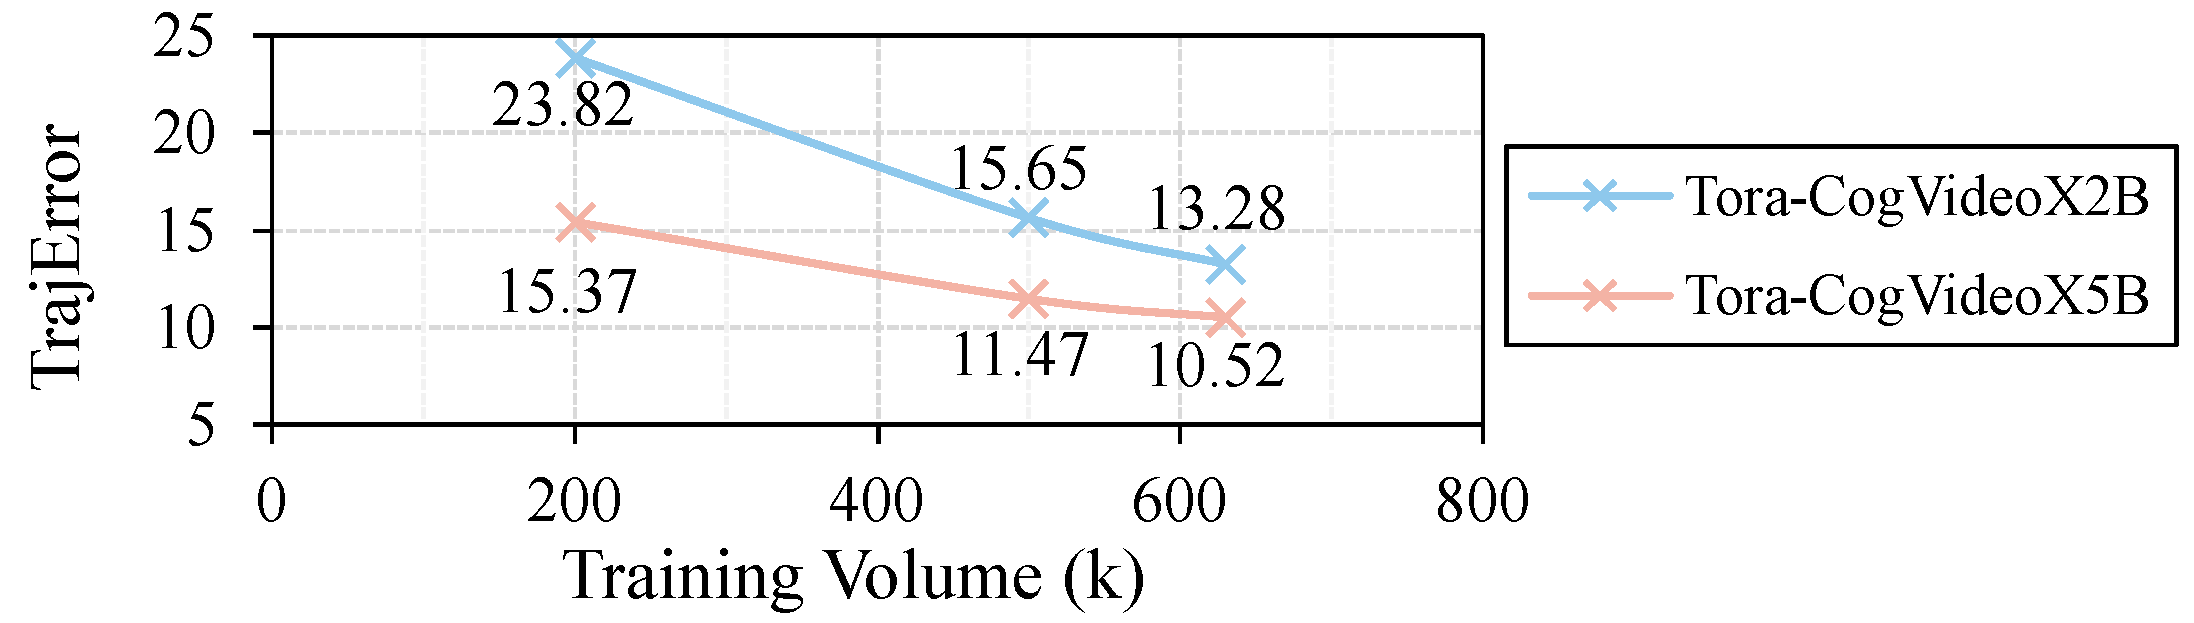
\includegraphics[width=1\linewidth]{images/reb-f1.pdf}
    \caption{Scaling Behavior of Motion Control Ability in Tora.}
    \label{f1}
    \vspace{-3mm}
\end{figure}

\noindent \textbf{(R2) Q4. Scaling ability of Tora.} Figure \ref{f1} depicts the scaling behavior of motion control ability, network complexity, and training data size. Tora was transferred to CogVideoX-2B and CogVideoX-5B with a data subset. The motion control ability aligns with scaling laws, integrating seamlessly with DiT scalability.

\noindent \textbf{(R1, R5) Q5. Universal DiT architecture.} Our proposed modules can be seamlessly integrated into the 3D full-attention DiT architecture. This approach is simple, yet effective and versatile. We demonstrate its effectiveness through visualizations in demo videos and the results presented in Table \ref{t1}.

\noindent \textbf{(R1, R3) Q6. Camera Control ability.} We found if trajectory points start with objects lacking regular movement patterns, such as sky, wood, or tables, Tora often generates camera movements to follow physical laws (see Figure 2 in paper and demo video). We recommend drawing trajectories within these objects for camera control and adding relevant camera details in text prompts to reduce ambiguity.

\noindent \textbf{(R3) Q7. Identity preservation ability.} We integrated ConsisID~[3] into our tuned CogVideoX-5B models. Since both module types use adapter-style training, we find it can directly achieve customization and motion control. With minimal fine-tuning, performance improves further.

\noindent \textbf{(R5) Q8. Fair comparisons with same training data.} We suggest using different training datasets generally might not significantly affect the fairness of comparisons. Methods like MotionCtrl, DragNUWA, and DragAnything all use their own training data, and DiT models are pretrained with diverse data for evaluation. Our curated training data enhances trajectory training, leading to better results.
%-------------------------------------------------------------------------





%%%%%%%%% REFERENCES
\noindent \textbf{References}

\tiny{
\setlength{\parindent}{0pt}
[1]~HunyuanVideo: A Systematic Framework For Large Video Generative Models. arXiv:2412.03603.

[2]~SAM 2: Segment Anything in Images and Videos. arXiv:2408.00714.

[3]~Identity-Preserving Text-to-Video Generation by Frequency Decomposition. arXiv:2411.17440.

}

% \newpage
% {
%     \small
%     \bibliographystyle{ieeenat_fullname}
%     \bibliography{main}
% }


\end{document}
